\section{Post-Mortem DDoS attack Analysis}

The primary goal of DDoSDB is build a large database with DDoS attacks. However


For a post-mortem analysis of the DDoS attack.

The goal of this section is to present how to extract only the attack vectors g
 
\begin{figure*}
	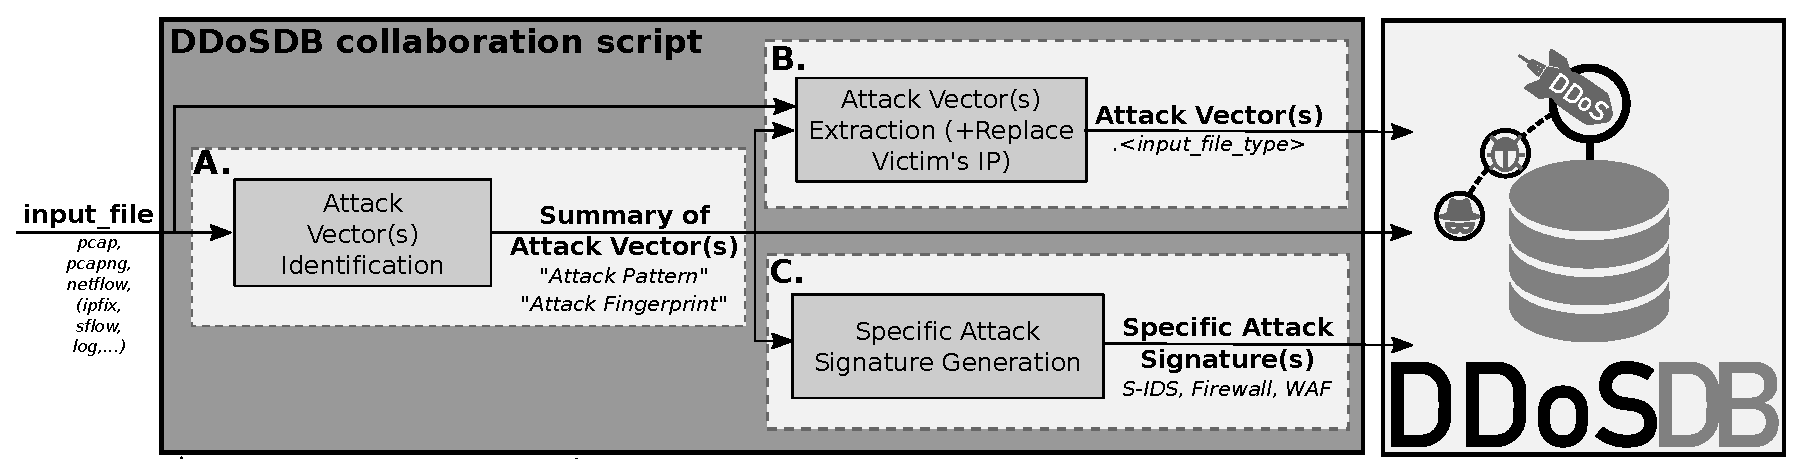
\includegraphics[width=\linewidth]{figs/workflow.eps}
	\caption{DDoSDB collaboration module}
	\label{fig:collaboration module}
\end{figure*}

The workflow for collaborating with DDoSDB is composed of three modules: (1) the attack vector identification, (2) the attack vector extraction, and (3) the DDoS signature generation for specific technologies. The attack vector identification module is the main module of the workflow. In this module the attack vectors of an DDoS attack are identified. The output of this module is a summary of the characteristics of each attack vector identified.

The attack vector identification is composed of consecutive analysis and filters. Given a network data collection (of several types: \eg .pcap, .pcapng, and .nfdump)

and replacement of the victim's IP address

Envisioning using these workflow in a ..., instead of 